\section{Il driver}

Il driver è stato sviluppato secondo le specifiche \emph{JDBC 4.0} (JSR 221) del Novembre 2006; secondo queste specifiche il driver è di tipo 4, ossia interamente scritto in java con accesso diretto alle risorse che compongono il database. Per aderire a queste specifiche ho parzialmente implementato le seguenti interfacce : 
\begin{itemize}
\item[-] java.sql.Driver (parziale)
\item[-] java.sql.DataSource (non implementata)
\item[-] java.sql.DatabaseMetaData (parziale)
\item[-] java.sql.ParameterMetaData (parziale)
\item[-] java.sql.ResultSetMetaData (parziale)
\item[-] java.sql.Wrapper (non implementata) 
\end{itemize}

In particolare il supporto al \emph{cursor} , alle transazioni , alle funzioni, al wrapping e alla creazione di strutture dati non è attualmente presente. Inoltre in Stantement non ho implementato la parte di PrepareStantement, quindi della figura sottostante [Fig.2] solo il ramo di sinistra è implementato e funzionante. 



\begin{figure}[ht]
\centering
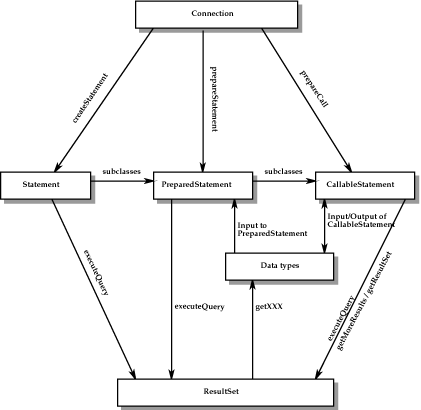
\includegraphics[width=1\textwidth]{immagini/jdbc.png}
\caption{JDBC Class Relationship}\label{fig:immagini/jdbc.png}
\end{figure}